\documentclass[letterpaper]{article}
\usepackage{graphicx}
\usepackage{subcaption}
\usepackage{tikz}
\usetikzlibrary{shapes.geometric, arrows}
\tikzstyle{startstop} = [rectangle, rounded corners, minimum width=3cm, minimum height=1cm,text centered, draw=black, fill=red!30]
\tikzstyle{io} = [trapezium, trapezium left angle=70, trapezium right angle=110, minimum width=3cm, minimum height=1cm, text centered, draw=black, fill=blue!30]
\tikzstyle{process} = [rectangle, minimum width=3cm, minimum height=1cm, text centered, draw=black, fill=orange!30]
\tikzstyle{decision} = [diamond, minimum width=3cm, minimum height=1cm, text centered, draw=black, fill=green!30]
\tikzstyle{arrow} = [thick, ->, >=stealth]

\title{Informe M\'etodos de Programaci\'on}
\date{04/2017}
\author{Paola Olgu\'in}

\begin{document}

  \pagenumbering{gobble}

  \maketitle{}

  \newpage

  \pagenumbering{arabic}

  \tableofcontents{}
  \newpage
  \section{Introducci\'on}
  Aqui va a ir la introduccion. Incluir informacion sobre Java, diagramas de flujo,
  diagramas de clase, diagramas de sucesion, programacion orientada a objetos.

  \subsection{Java}
  Blablablablabla

  \subsection{Diagramas}
  \newpage
  \subsubsection{Flujo}
  \begin{figure}[h]
    \begin{subfigure}{0.99\textwidth}
    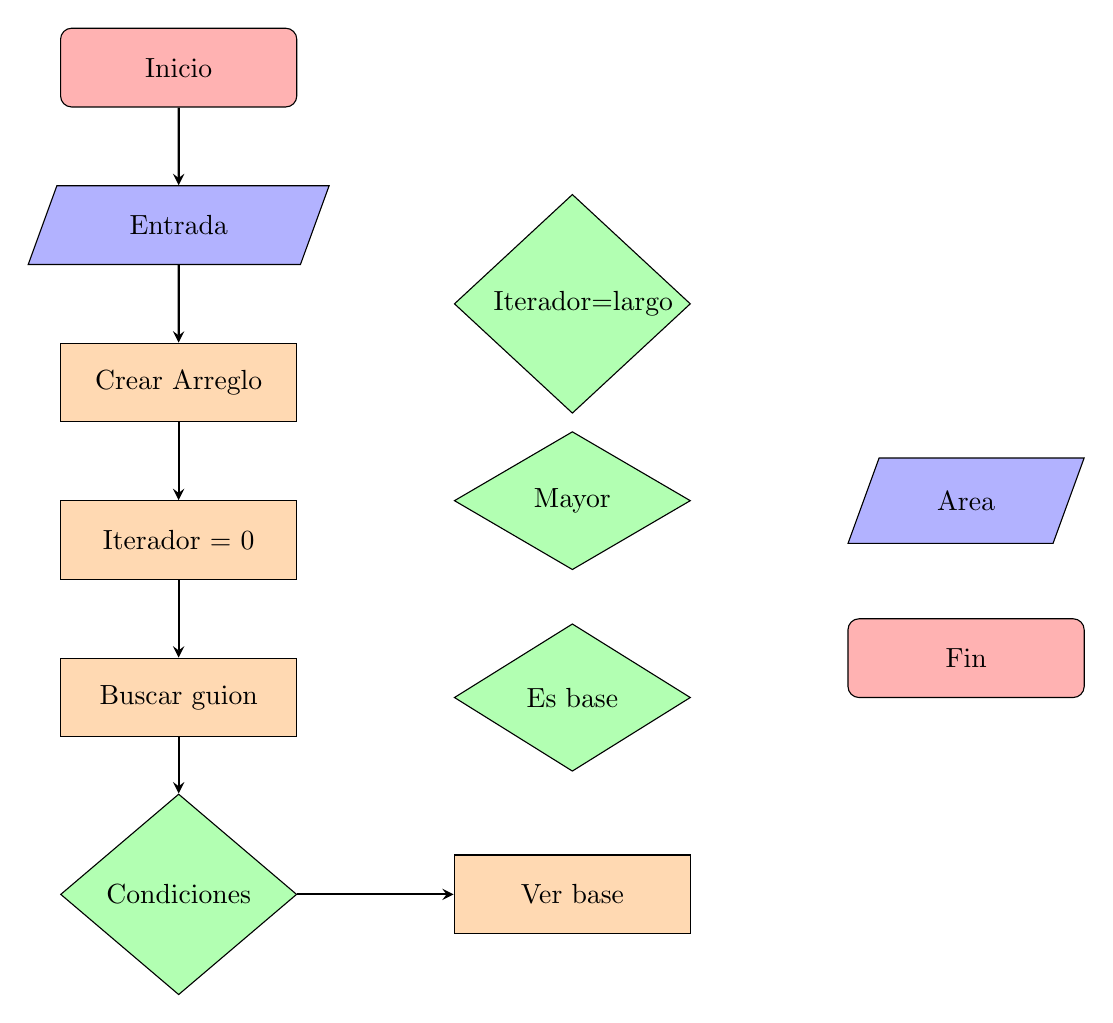
\begin{tikzpicture}[node distance = 2cm]
      \node (inicio) [startstop] {Inicio};
      \node (in1) [io, below of=inicio] {Entrada};
      \node (pro1) [process, below of=in1] {Crear Arreglo};
      \node (pro2) [process, below of=pro1] {Iterador = 0};
      \node (pro3) [process, below of=pro2] {Buscar guion};
      \node (dec1) [decision, below of=pro3, yshift = -0.5cm] {Condiciones};
      \node (pro4) [process, right of=dec1, xshift=3cm] {Ver base};
      \node (dec2) [decision, above of=pro4, yshift = 0.5cm]{Es base};
      \node (dec3) [decision, above of=dec2, yshift=0.5cm]{Mayor};
      \node (dec4) [decision, above of=dec3, yshift=0.5cm, text centered, text width=2cm]{Iterador=largo};
      \node (out1) [io, right of=dec3, xshift=3cm]{Area};
      \node (fin) [startstop, below of= out1] {Fin};
      \draw [arrow] (inicio) -- (in1);
      \draw [arrow] (in1) -- (pro1);
      \draw [arrow] (pro1) -- (pro2);
      \draw [arrow] (pro2) -- (pro3);
      \draw [arrow] (pro3) -- (dec1);
      \draw [arrow] (dec1) -- (pro4);
    \end{tikzpicture}
    \caption{Diagrama Iterativo}
    \end{subfigure}
  \end{figure}
  \newpage
  \subsubsection{Clase}
  \subsubsection{Sucesi\'on}
  \subsection{Programaci\'on Orientada a Objetos}
  \newpage
  \section{Descripci\'on del problema}

  \par
  El problema a solucionar es el de, dado un tri\'angulo de n filas,
  formado por tri\'angulos m\'as peque\~nos de color negro y blanco, hallar si hay
  tri\'angulos formados \'unicamente de tri\'angulos blancos dentro del tri\'angulo
  mayor. Si se encuentra m\'as de uno, reconocer el mayor, e imprimir por pantalla
  que el tri\'angulo es de \'area a; donde a es la suma de todos los blancos que
  componen el tri\'angulo hallado.\par

    \begin{figure}[h!]
      \centering
      \includegraphics[scale = 0.5, angle = 180]{triangulo1}
      \caption{Ejemplo}
    \end{figure}

  Para menor confusi\'on, se hablar\'a de tri\'angulo mayor para
  referirnos al tri\'angulo formado por los menores de ambos colores, tri\'angulo
  blanco para referirnos al mayor tri\'angulo formado \'unicamente por blancos, y
  tri\'angulos menores para los de menor tama\~no.\par

  Para poder analizar bien el problema, se tom\'o en cuenta ciertas
  consideraciones que se mencionar\'an a continuaci\'on:
    \begin{itemize}
    \item Las filas son de un n\'umero impar de tri\'angulos menores,
    lo cual implica que la mayor \'area posible va a ser \(n^2\), con \(n\) siendo el
    n\'umero de filas del tri\'angulo mayor, y la menor \'area posible ser\'a 0,
    en el caso que el tri\'angulo mayor se componga \'unicamente de tri\'angulos
    negros. Esto puesto que $\sum_{i=0}^{n} 2{i}+1 = {n}^2$
    \item Teniendo lo anterior en mente, si en la fila \(n-1\) (considerando la
    primera como 0), nos encontramos un tri\'angulo negro, sabemos enseguida
    que la mayor \'area ya no puede ser \({n}^2\), sino que \({(n-1)}^2\). Esto, sin embargo,
    no nos dice demasiado, siendo que el tri\'angulo blanco puede formarse hacia
    arriba (hacia la base) o hacia abajo (la punta), y puede formarse por
    partes de filas sin considerarlas enteras.
    \item Retomando la consideraci\'on, puesto que las filas que componen el
    tri\'angulo mayor son todas impares, ning\'un tri\'angulo blanco puede tener
    una fila con un n\'umero par de tri\'angulos menores.
    \item Cada fila empieza y termina con un tri\'angulo hacia la punta, lo que
    implica que los \'indices pares de las filas apuntan en esa direcci\'on y
    los \'indices impares apuntan hacia la base. La direcci\'on de un tri\'angulo
    se define, entonces, por hacia donde apuntan los extremos de la base, o,
    en su defecto, hacia donde mira la punta.
    \item Cada fila m\'as grande, tiene dos elementos m\'as que la
    anterior.
    \item Se consideran como tri\'angulos \'unicamente los que ser\'ian un
    tri\'angulo que nosotros podamos reconocer visualmente. Por
    lo tanto en un c\'odigo como el de la figura \ref{subfig:notriangulo} reconocer\'ia un
    \'area de uno, puesto que su representaci\'on gr\'afica no nos
    muestra un tri\'angulo. En cambio, uno como el de la figura \ref{subfig:rialtriangulo} reconocer\'ia un\'area de cuatro.
    \end{itemize}

    % No se como hacer que estas imagenes se pongan bien
    \begin{figure}
      \centering
      \begin{subfigure}{0.45\textwidth}
        \includegraphics[width=0.7\linewidth]{rialtriangulo}
        \caption{Tri\'angulo blanco mayor con \'area 4.}
        \label{subfig:rialtriangulo}
      \end{subfigure}
      \begin{subfigure}{0.45\textwidth}
        \includegraphics[width=0.7\linewidth]{notriangulo}
        \caption{Tri\'angulo blanco mayor corresponde a un \'unico tri\'angulo peque\~no}
        \label{subfig:notriangulo}
      \end{subfigure}
      \caption{Visualizaci\'on}
    \end{figure}

  \newpage
  \section{Descrici\'on de la Soluci\'on}
  El proyecto pide el desarrollo de dos algoritmos de resoluci\'on, uno iterativo
  y otro recursivo. Se partir\'a hablando del primero, puesto que es el m\'as trivial
  de ver.
  \subsection{Iteraci\'on}
  La iteraci\'on se define como el acto de repetir un proceso. Esto, aplicado a las
  ciencias de la computaci\'on o la programaci\'on repercute en un ciclo, durante
  el cual se repite una cierta acci\'on.\par
  En el caso del problema propuesto, la soluci\'on iterativa se pens\'o como si
  se estuviera viendo un tri\'angulo cualquiera y se busc\'o la forma m\'as trivial
  para encontrar los mayores tri\'angulos blancos.\par
  La forma m\'as obvia es ir contando uno a uno los tri\'angulos blancos que forman
  otro mayor, y comparar, de estos, cual tiene un \'area mayor. Sin embargo, esta
  forma se vuelve muy poco eficiente para un tri\'angulo de muchas filas, puesto
  que se estar\'ia sumando uno a uno los tri\'angulos peque\~nos, para luego almacenar
  cada cantidad obtenida para sacar la mayor entre ellas. Adem\'as hemos de considerar
  que un programa no tiene c\'omo ver si algo es un tri\'angulo o no. Por eso, gracias
  a las consideraciones tomadas anteriormente podemos optimizar un poco la b\'usqueda.
  \begin{enumerate}
    \item Como un tri\'angulo, en cada fila, s\'olo puede tener un n\'umero impar de
    tri\'angulos menores, basta con saber el n\'umero de filas para saber el \'area.
    \item Como la direcci\'on la define la punta, y \'esta de por si corresponde a
    un tri\'angulo de los peque\~nos, con encontrar \'esta nos basta, pues el resto de la
    figura se puede formar a partir de ah\'i.
    \item Cada fila mayor, es dos tri\'angulos m\'as larga que la anterior.
    \item En lugar de almacenar todas las \'areas que encontremos, almacenamos la
    mayor hasta el momento y seguimos buscando; si se encuentra un \'area mayor, se
    reemplaza, si no, se mantiene la actual. Como las \'areas ser\'an siempre un
    n\'umero entero no negativo, empezamos considerando un \'area de cero.
  \end{enumerate}
\subsubsection{Proceso}
Para cualquier entrada que tengamos, se hace un arreglo con el tri\'angulo mayor,
tal que cada fila de \'este es un elemento en el arreglo. Luego, se recorre el
arreglo, pasando por cada fila de la figura. En \'estas, se busca \'unicamente guiones,
que representan nuestros tri\'angulos menores blancos. Dichos tri\'angulos se toman
como una punta del tri\'angulo blanco, por lo que nos faltar\'ia ver si le podemos
dar una base. Cabe mencionar que con hallar una punta, ya tenemos un \'area de 1.\par
Como se buscan tri\'angulos dentro del original que obtuvimos, tenemos que asegurar
que la posible base no se salga del tri\'angulo como en la figura \ref{fig:baseafuera}.
Esto se hace teniendo en mente la consideraci\'on antes mencionada; que con dos
tri\'angulos m\'as se aumenta una fila. Entonces, dependiendo del sentido de la
punta encontrada (dado por la paridad del \'indice donde fue encontrada), se ve
que la base del tri\'angulo blanco no sea m\'as grande que la del tri\'angulo
mayor, que el largo de la base sea menor que los l\'imites del mayor, y que, en
el caso que la punta vea hacia la base del tri\'angulo mayor (\'indice impar), no
nos pasemos de la punta del original.\par
Una vez cumplidas esas condiciones, tenemos que ver que tengamos una base blanca,
efectivamente. Como sabemos la fila en la que encontramos la punta, y que, de nuevo,
una fila m\'as grande implica dos tri\'angulos m\'as, podemos calcular la cantidad
de tri\'angulos menores que deber\'iamos encontrar en la base. Teniendo esta
cantidad, podemos crear una base blanca y comparar si es lo mismo que tenemos bajo
la punta hallada. Ya que cada fila corresponde a un string, se pueden dividir en
substrings, esto es lo que se hace para verificar que estemos viendo una base
blanca; se compara un string formado s\'olo de guiones con el substring de lo que
ser\'ia la base de la punta.
  \begin{figure}[t!]
    \centering
    \includegraphics[scale = 0.7]{baseafuera}
    \caption{Posible tri\'angulo blanco con base afuera del tri\'angulo mayor.}
    \label{fig:baseafuera}
  \end{figure}
  \par Como tenemos una iteraci\'on, la cantidad de veces que logremos aumentar
  (o disminuir) filas, corresponde a la cantidad de filas que tendr\'a el
  tri\'angulo blanco, por lo que simplemente elevamos este n\'umero al cuadrado
  para sacar el \'area correspondiente. Luego, se compara con el n\'umero que
  tenemos guardado, reemplaz\'andolo dependiendo de si es menor o mayor que el
  cuadrado obtenido.

\end{document}
